\documentclass[12pt,a4paper]{article}
\usepackage[utf8]{inputenc}
\usepackage[brazil]{babel}
\usepackage{graphicx}
\usepackage{amssymb, amsfonts, amsmath}
\usepackage{color}
\usepackage{float}
\usepackage{enumerate}
%\usepackage{subfigure}
\usepackage[top=2.5cm, bottom=2.5cm, left=1.25cm, right=1.25cm]{geometry}

\newcommand{\sen}{\,\textrm{sen}\,}
\newcommand{\tg}{\,\textrm{tg}\,}

\begin{document}
\pagestyle{empty}

\begin{center}
\begin{tabular}{ccc}
\begin{tabular}{c}

\includegraphics[scale=0.25]{../../biblioteca/imagem/brasao-de-armas-brasil} \\
\end{tabular} & 
\begin{tabular}{c}
Ministério da Educação \\
Universidade Federal dos Vales do Jequitinhonha e Mucuri \\
Faculdade de Ciências Sociais, Aplicadas e Exatas - FACSAE \\
Departamento de Ciências Exatas - DCEX \\
Disciplina: Cálculo Numérico\\
Prof.: Luiz C. M. de Aquino\\
\end{tabular} &
\begin{tabular}{c}

\includegraphics[scale=0.25]{../../biblioteca/imagem/logo-ufvjm} \\
\end{tabular}
\end{tabular}

Aluno(a): \rule{0.5\textwidth}{0.01cm} \quad Data: \rule{0.6cm}{0.01cm} / \rule{0.6cm}{0.01cm} / \rule{1.25cm}{0.01cm}
\end{center}

\begin{center}
 \textbf{Avaliação II}
\end{center}

\textbf{Instruções}
\begin{itemize}
 \item Todas as justificativas necessárias na solução de cada questão devem estar presentes nesta avaliação;
 \item As respostas finais de cada questão devem estar escritas de caneta;
 \item Esta avaliação tem um total de 25,0 pontos.
\end{itemize}

\begin{enumerate}
 \item \textbf{[7,5 pontos]} Considere o problema do circuito hidráulico mostrado na Figura~\ref{fig:tub}. Este sistema está alimentado por 
um reservatório cuja a pressão é mantida constante e igual a $P_r = 10$. As saídas das tubulações desembocam na atmosfera, onde a pressão é 
considerada nula (isto é, $P_a = 0$). Deste modo, a vazão $Q_i$ da $i$-ésima tubulação depende da diferença de pressão $\Delta P_i$ 
de tal modo que $Q_i = K_iL_i\Delta P_i,$ onde $K_i$ é a resistência hidráulica e $L_i$ o comprimento da tubulação. Por exemplo, para a 
tubulação $8$ temos que $Q_8 = K_8L_8\Delta P_8$, sendo que $\Delta P_8 = P_1 - P_4$ (ou seja, a pressão que ``entra'' na tubulação pela 
bifurcação $1$ menos a pressão que ``sai'' da tubulação pela bifurcação $4$). Por outro lado, sabe-se que em cada bifurcação a soma das vazões 
deve ser nula. Por exemplo, na bifurcação $4$ temos que $Q_8 - Q_6 - Q_7 = 0$ (aqui note que a vazão que ``entra'' na bifurcação é considerada positiva, 
enquanto que a que ``sai'' é considerada negativa). Considerando essas informações e os dados da Tabela~\ref{tab:dados}, responda aos quesitos abaixo.

\begin{figure}[H]
 \centering
 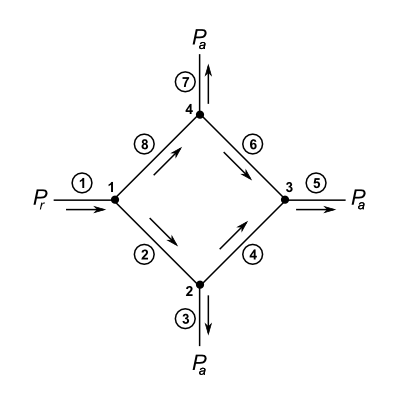
\includegraphics[scale=0.7]{imagem/Tubulacao.png}
 \caption{Esquema do circuito hidráulico.}
 \label{fig:tub}
\end{figure}

\begin{table}[H]
 \centering
 \begin{tabular}{c|c|c}
  Tubulação $i$ & $K_i$ & $L_i$ \\ \hline
  1 & 0,02 & 1,0 \\ \hline
  2 & 0,005 & 2,0 \\ \hline
  3 & 0,085 & 0,5 \\ \hline
  4 & 0,02 & 1,0 \\ \hline
  5 & 0,075 & 0,5 \\ \hline
  6 & 0,085 & 0,5 \\ \hline
  7 & 0,015 & 2,0 \\ \hline
  8 & 0,01 & 1,0 
 \end{tabular}
 \caption{Resistência hidráulica e comprimento das tubulações.}
 \label{tab:dados}
\end{table}

\begin{enumerate}
 \item Arme o sistema de equações necessário para obter as pressões em cada bifurcação.
 \item Explique o procedimento necessário para resolver o sistema do quesito (a) usando Eliminação Gaussiana. Atenção: não é necessário determinar a solução do sistema. 
\end{enumerate}

 \item \textbf{[2,5 pontos]} Suponha que uma matriz $A$ foi fatorada no formato $LU$. Preencha os espaços em branco abaixo de modo a determinar 
as matrizes $A$, $L$ e $U$.

$$
A = \begin{bmatrix}\square & \square & \square \\ 1 & 0 & \square \\ \square & -4 & -3\end{bmatrix};\,  
L = \begin{bmatrix}\square & 0 & 0 \\ \square & \square & 0 \\ -5 & \square & \square\end{bmatrix};\, 
U = \begin{bmatrix}-2 & \square & 4 \\ 0 & \square & 3 \\ 0 & 0 & -1\end{bmatrix}
$$

 \item \textbf{[5,0 pontos]} Considere o seguinte sistema de equações:
  $$%x = -1, y = 1, z = 2.
   \begin{cases}
    2x - 4y + 8z  - w = -6 \\
    -2x  - 2y + z - 7w = -5 \\
    5x  - y + z - 2w = -2 \\
    x - 4y - z + w = 8
   \end{cases}
  $$

  \begin{enumerate}
   
   \item Da forma como ele está arrumado, é recomendável usar diretamente o método de Gauss-Jaboci? Justifique sua resposta.
   \item Exiba as equações utilizadas pelo método de Gauss-Jacobi para obter uma solução aproximada desse sistema.
   \item Exiba as equações utilizadas pelo método de Gauss-Seidel para obter uma solução aproximada desse sistema.
  \end{enumerate}

 \item \textbf{[5,0 pontos]} Considere um sistema de equações lineares com três equações e três incógnitas. Suponha que é possível aplicar o 
Método de Gauss-Jacobi nesse sistema com garantia de convergência. Determine as matrizes $x^{(k)}$, $B$ e $c$ de tal modo a escrever este método 
no formato $x^{(k+1)} = Bx^{(k)} + c$.

 \item \textbf{[5,0 pontos]} Determine a fatoração $LU$ da matriz $A = \begin{bmatrix} a & b \\ c & d\end{bmatrix}$. Use essa fatoração para obter 
a solução do sistema $Ax = y$, onde $x = \begin{bmatrix} x_1 \\ x_2 \end{bmatrix}$ e $y = \begin{bmatrix} y_1 \\ y_2\end{bmatrix}$.

\end{enumerate}
\end{document}
